\chapter{Ausgewählte Aspekte}

\section{NGINX sichern mit letsencrypt}

\section{EspWifiManager Implementation}

\section{Die Wichtigkeit von Erase Flash}

\section{ELF vs Bin}

\subsection{ELF}

ELF ist die Abkürzung für Executable and Linkable Format und definiert die Struktur für Binärdateien, Bibliotheken und Core-Dateien. Die formale Spezifikation ermöglicht es dem Betriebssystem, die zugrunde liegenden Maschinenanweisungen korrekt zu interpretieren. ELF-Dateien sind normalerweise die Ausgabe eines Compilers oder Linkers und haben ein Binärformat.
\newline
\newline
Ein häufiges Missverständnis ist, dass ELF-Dateien nur für Binärdateien oder ausführbare Dateien bestimmt sind. Es ist jedoch möglich sie für Teilstücke (Objektcode) verwendet zu können. Ein weiteres Beispiel sind gemeinsam genutzte Bibliotheken oder sogar Core-Dumps (Core- oder a.out-Dateien). Die ELF-Spezifikation wird auch unter Linux für den Kernel selbst und die Linux-Kernelmodule verwendet.


\subsection{Struktur}
Aufgrund des erweiterbaren Designs von ELF-Dateien unterscheidet sich die Struktur je nach Datei. Eine ELF-Datei besteht aus:

 
\subsection{ELF-Header}
Dateidaten
Mit dem Befehl readelf können wir uns die Struktur einer Datei ansehen und sie sieht ungefähr so aus:

\begin{figure}[H]
    \begin{center}
        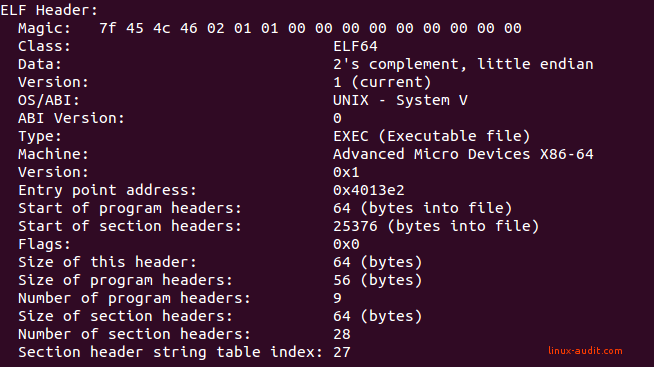
\includegraphics[scale=0.5]{images/elf-header-linux-binary.png}
        \caption{Details einer Elf-binary \cite{details_of_Elf_binary}}
    \end{center}
\end{figure}
 
\subsection{ELF-Header}
Wie in diesem Screenshot zu sehen ist, beginnt der ELF-Header mit etwas Magic. Diese ELF-Header-Magic liefert Informationen über die Datei. Die ersten 4 hexadezimalen Teile definieren, dass dies eine ELF-Datei ist (45 = E, 4c = L, 46 = F), der der Wert 7f vorangestellt ist.
 
Dieser ELF-Header ist obligatorisch. Es stellt sicher, dass Daten während der Verknüpfung oder Ausführung korrekt interpretiert werden. Um die innere Funktionsweise einer ELF-Datei besser zu verstehen, ist es hilfreich zu wissen, dass diese Header-Informationen verwendet werden.
 
\subsection{Class}
Nach der ELF-Typdeklaration ist ein Class-feld definiert. Dieser Wert bestimmt die Architektur für die Datei. Es kann sich um eine 32-Bit- (= 01) oder 64-Bit- (= 02) Architektur handeln. Magic zeigt eine 02, die vom Befehl readelf als ELF64-Datei übersetzt wird. Mit anderen Worten, eine ELF-Datei, die die 64-Bit-Architektur verwendet.

\subsection{Data}
Der nächste Teil ist das Data-feld. Es kennt zwei Optionen: 01 für LSB (Least Significant Bit), auch als Little-Endian bekannt. Dann gibt es den Wert 02 für MSB (Most Significant Bit, Big-Endian). Dieser spezielle Wert hilft dabei, die verbleibenden Objekte in der Datei korrekt zu interpretieren. Dies ist wichtig, da verschiedene Prozessortypen unterschiedlich mit den eingehenden Anweisungen und Datenstrukturen umgehen. In diesem Fall wird LSB verwendet, was für Prozessoren vom Typ AMD64 üblich ist.